\documentclass[12pt]{article}

\author{Corbin T. Rochelle}
\title{Lab 2 Write-Up}
\date{\today}

\usepackage{geometry}
 \geometry{
 a4paper,
 total={170mm,257mm},
 left=20mm,
 top=20mm,
 }

\usepackage{graphicx}
\usepackage{listings}

\begin{document}

\maketitle

\section{Describe, in a few sentences, the development process you used during this assignment. In what order did you develop the parsing functions? How many functions did you write?}

The first thing I did was read what was already included in the starting files to try to see what needed to be developed and what was already written.
After understanding what I needed to do, I defined the structures in my parser.h file that I expected I would need. 
After that I defined the structures in parser.c, starting with the noun and adjective phrases, then moving to the verb phrases. 
After getting the base code written I tested it against all of the correct input files (considering I had not coded error checking yet) and worked on it until the output information was correct.
I then worked for more time than I expected to get the spacing to be correct so that diff would yield no output for the correct files.
I then looked at all of the invalid input options so that all of the error checking could be correct. 
In the end I defined five extra functions: noun\_phrase(), verb\_phrase(), adjective\_phrase(), spacer(), and firstOf\_sentence(). 

\section{Consider the diagrammed sentences in the file Parse\_Tree\_Examples.pdf. Invent your own test input sentence, which parses correctly, and draw a similar parse tree diagram of this sentence. (Your tree may be drawn by hand and scanned.) Also list your code's output for this test input sentence.}

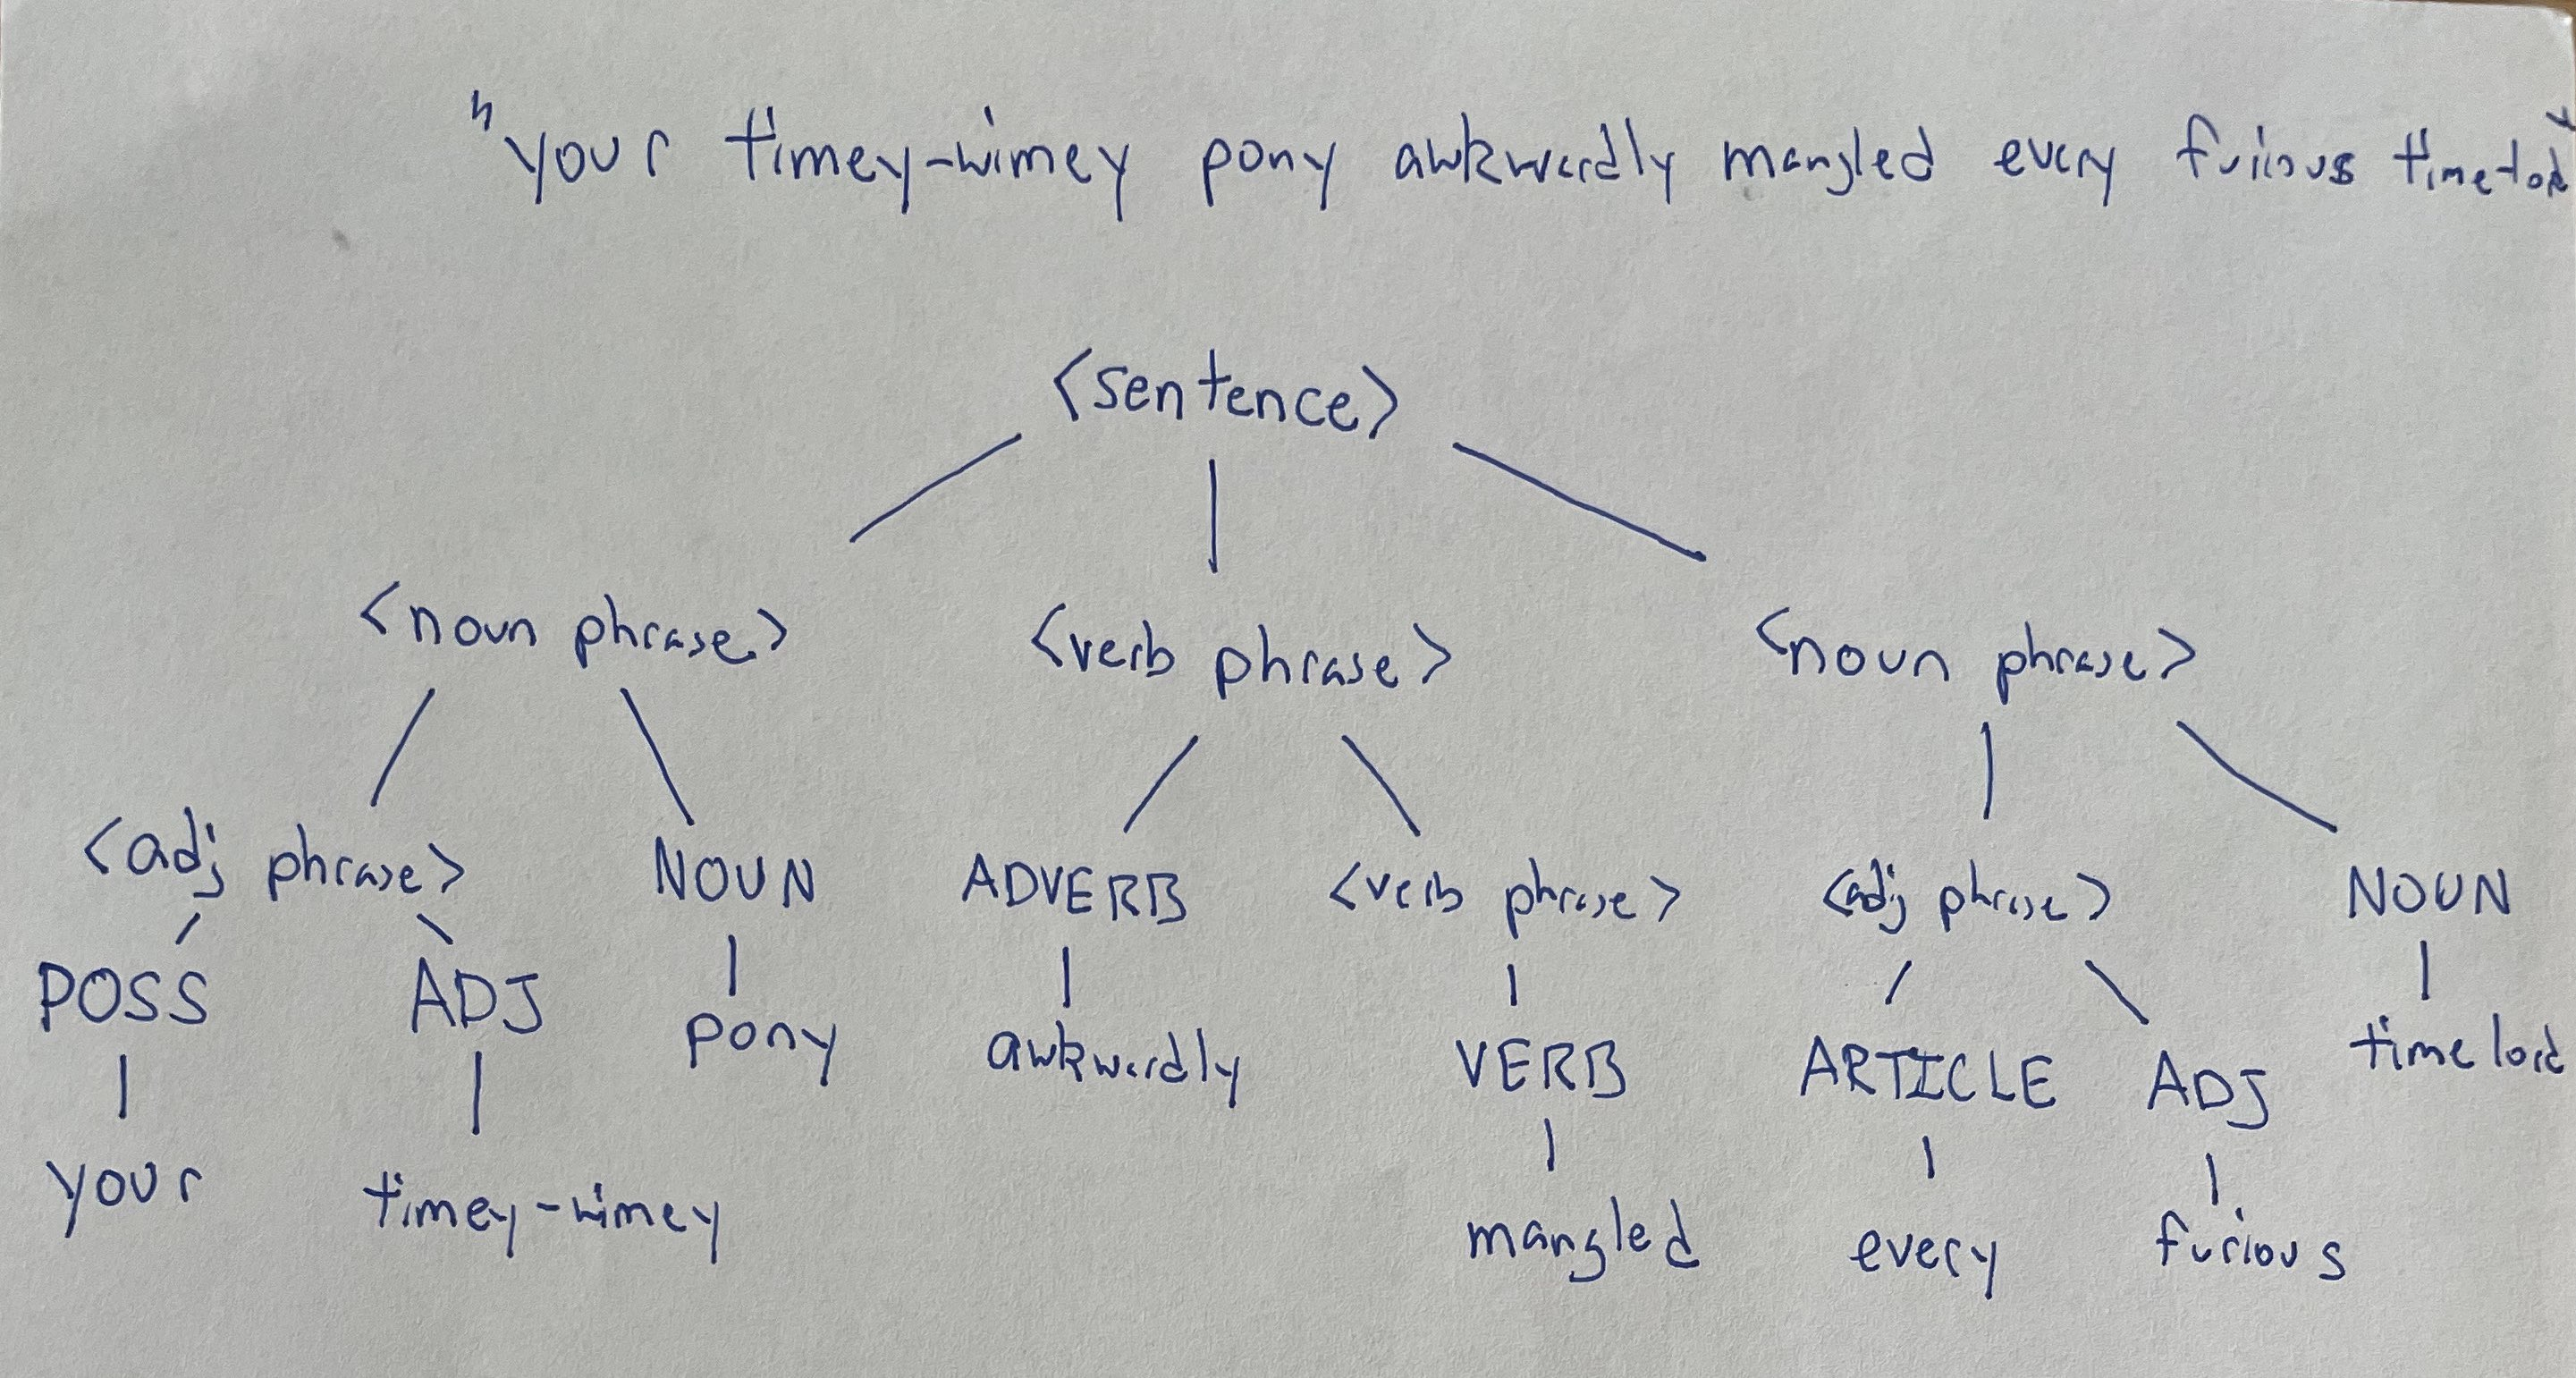
\includegraphics[width=\textwidth]{diagram.jpeg}

Listed next is the output for the parse tree's input:
\lstinputlisting{test.correct}

\section{Discuss the role of the program call stack in the parsing process. Which one of the test input sentences resulted in the deepest call stack? Why was it this deep?}

The call stack in an important process to look at in this program because it is a top-down parser, which involves breaking a complex structure down into its simplest component parts. 
The input file that had the deepest call stack was input5.in. 
This is because it takes advantage of the recursive nature of the <verb phrase> function.
Potentially, this function can infinitely call itself, creating an infinitely deep call stack. 
In input.5's case, it recursive calls <verb phrase> five times, which is the deepest call stack for a <noun phrase> or <verb phrase>.
Looking at the call stack depth from the <sentence>, the depth of this <verb phrase> stack is seven. 

\section{Describe, in a few sentences, any sources you consulted during your development of this assignment.}

The only sources I used in this project is the starter files given in the project and the driver file for Lab 1, to understand how to call tokens and strings from lex(). 

\end{document}
